\documentclass[11pt]{article}
\usepackage{amsmath, amsthm, amssymb, fancyhdr, fancybox, graphicx}
\usepackage{psfrag, dcolumn, bm, accents, setspace, textcomp}
\usepackage{url, hyperref, color, wasysym}
\usepackage{dsfont}
\usepackage{booktabs}

\pagestyle{empty}

\oddsidemargin  0.05in
%\evensidemargin  7pt
\marginparsep 0pt
\topmargin=-0.5in
\textwidth=6.42in
\textheight=9in
\parskip = 3pt plus 1pt minus 1pt

\newtheorem{thm}{Theorem}
\newtheorem{lemma}{Lemma}
\newtheorem{corollary}{Corollary}
\newtheorem{identity}{Identity}
\newtheorem{defn}{Definition}
\newtheorem{algorithm}{Algorithm}
\newcommand{\argmax}{\operatornamewithlimits{argmax}}
\newcommand{\argmin}{\operatornamewithlimits{argmin}}
\newcommand{\dist}{\operatornamewithlimits{\sim}}
\newcommand{\converges}{\operatornamewithlimits{\longrightarrow}}
\newcommand{\cprob}{\stackrel{p}{\longrightarrow}}
\newcommand{\cdist}{\stackrel{d}{\longrightarrow}}
\newcommand{\cprobanddist}{\stackrel{p,d}{\longrightarrow}}
\newcommand{\cas}{\stackrel{a.s.}{\longrightarrow}}
\newcommand{\crth}{\stackrel{r}{\longrightarrow}}
\newcommand{\cone}{\stackrel{1}{\longrightarrow}}
\newcommand{\cms}{\stackrel{m.s.}{\longrightarrow}}
\newcommand{\iid}{\stackrel{iid}{\sim}}
\newcommand{\wtssim}{\stackrel{wts}{\sim}}
\newcommand{\simind}{\stackrel{ind}{\sim}}
\newcommand{\eqas}{\stackrel{a.s.}{=}}
\newcommand{\eqdist}{\stackrel{d}{=}}
\def\Var{\textrm{Var}\,}
\def\E{\mathbb{E}\,}
\def\Wish{\textrm{Wishart}\,}
\def\IWish{\textrm{Inv-Wishart}\,}
\def\Pois{\textrm{Poisson}\,}
\def\Nb{\textrm{Neg-Bin}\,}
\def\Gm{\textrm{Gamma}\,}
\def\Expo{\textrm{Expo}\,}
\def\Beta{\textrm{Beta}\,}
\def\Pareto{\textrm{Pareto}\,}
\def\Unif{\textrm{Uniform}\,}
\def\Ber{\textrm{Bernoulli}\,}
\def\Bin{\textrm{Binomial}\,}
\def\s{\mathbf{s}}
\def\Y{\mathbf{Y}}
\def\F{\mathbf{F}}
\def\Ft{\mathbf{F}^{T}}
\def\G{\mathbf{G}}
\def\V{\mathbf{V}}
\def\W{\mathbf{W}}
\def\xt{\mathbf{x}^{T}}
\def\kron{\otimes\,}
\def\R{R} % May change this
\def\G{G} % May change this
\def\I{\mathbb{I}}
\def\J{\mathbb{J}}
\def\1{\mathbf{1}}
\def\0{\mathbf{0}}
\def\R{\texttt{R}}
\def\lme{\texttt{lme4}}
\def\lmer{\texttt{lmer}}
\def\Xi{X_{i}}
\def\Zi{Z_{i}}
\def\diag{\textrm{diag}}
\def\bdiag{\textrm{block-diag}}
\def\dim{\textrm{dim}}
\def\tr{\textrm{tr}}
\def\nstat{n_{\textrm{stations}}}
\def\nrcm{n_{\textrm{RCM}}}
\def\ngcm{n_{\textrm{GCM}}}
\def\ngrid{n_{\textrm{grid}}}

\def\lNS{$\log(N)-\log(S)$}
\def\apl{\alpha_{PL}}
\def\bpl{\beta_{PL}}
\def\Sstar{S_{*}}
\def\Smin{S_{min}}
\def\Yobs{Y_{obs}}
\def\Ymis{Y_{mis}}
\def\Nobs{N_{obs}}
\def\Nmis{N_{mis}}
\def\Ncom{N_{com}}
\def\Iobs{I_{obs}}
\def\Imis{I_{mis}}
\def\Icom{I_{com}}
\def\Sobs{S_{obs}}
\def\Smis{S_{mis}}
\def\Scom{S_{com}}
\def\Eobs{E_{obs}}
\def\Emis{E_{mis}}
\def\Ecom{E_{com}}
\def\Lobs{L_{obs}}
\def\Lmis{L_{mis}}
\def\Lcom{L_{com}}

\def\CUDA{\texttt{CUDA}\,}
\def\Python{\texttt{Python}\,}
\def\PyCUDA{\texttt{PyCUDA}\,}
\def\numpy{\texttt{numpy}\,}
\def\OpenCL{\texttt{OpenCL}\,}
\def\GPUArray{\texttt{GPUArray}\,}

\newcommand{\df}[1]{ \mathop{\mathrm{d}#1} }

\begin{document}

\title{Nested Sampling and the Evaluation of the \lq{}Evidence\rq{} for Bayesian Model Selection}
\author{
Paul D. Baines, Nicholas Ulle\\
\emph{University of California, Davis}
}
\date{\today}
\maketitle

\section{Introduction}\label{overview}
A popular Bayesian model selection strategy is comparison of the 
``evidence'' for each model.
That is, the average likelihood over the prior probability space.
This is quite intuitive---models with greater evidence are a better fit for
the data.
Here we will focus solely on methods for evaluating the evidence.

Formally, for likelihood~$L$ and prior~$\pi$, the evidence is defined as
\[
    Z(y) = \int L(y; \theta) \pi(\theta) \df{\theta}.
\]
This expression is deceptively simple-looking;
in practice, direct evaluation is often impractical or impossible,
because the prior parameter $\theta$ is multi-dimensional.

Nested sampling overcomes this difficulty by recasting the problem,
to arrive at a one-dimensional integral which can the be evaluated using
standard methods from numerical analysis.
Consider the random variable $L(y; \theta) \geq 0$,
which has survival function
\[
    S(\lambda) = \Pr_\pi \bigl[ L(y; \theta) > \lambda \bigr].
\]
A well-known result is that the integral of the survival function of a
non-negative random variable is its expectation. In this case,
\[
    Z(y)
    =
    \E_\pi \bigl[ L(y; \theta) \bigr]
    =
    \int_0^\infty S(\lambda) \df{\lambda}.
\]
Since $S$ is monotonic, this area is the same as
% TODO Possibly insert figure showing this.
\[
    Z(y)
    =
    \int_0^1 S^{-1}(x) \df{x},
\]
where $S^{-1}$ is the upper quantile function of $L(y; \theta)$.
Explicit evaluation of $S^{-1}$ may be quite challenging,
but we can avoid this entirely.
% TODO Clarify this explanation a bit.
Instead, we sample $n$ values $\theta_1, \ldots, \theta_n$
from the prior~$\pi$, and define $L_i = L(y; \theta_i)$,
for $i = 1, \ldots, n$.
The smallest among these, $L_{(1)}$,
is an estimate of the $(1 - 1 / n)$ upper quantile.
If we remove $L_{(1)}$ from the sample and replace it with a new point
drawn in the same way, but constrained to be strictly greater,
then the new $L_{(1)}$ is an estimate of the $(1 - 1/n)^2$ upper quantile.
By proceeding in this fashion, we can estimate $S^{-1}$ over its entire
domain.
It's then straightforward to approximate the integral numerically.

Here we have implemented the nested sampler and applied it to a
toy example where the evidence can also be computed analytically.
We also propose a mixture model, where the evidence cannot be computed
analytically, for further study, including the use of alternative
estimators of the evidence.

\section{Toy Example}
Let:
\begin{align*}
Y_{i} \sim{} N(\mu,\sigma^{2}) , \qquad i=1,\ldots,n ,
\end{align*}
with prior $p(\mu)\propto{}N(\mu_{0},\tau_{0}^{2})$ and $\sigma^{2}$ known. 

Letting $C=(2\pi)^{-(n+1)/2}(\tau_{0}^{2})^{-1/2}(\sigma^{2})^{-n/2}$, the evidence, or marginal likelihood, is:
\begin{align*}
 p(y) &= \int p(y_{1},\ldots,y_{n}|\mu)p(\mu)d\mu = \int p(\mu)\prod_{i=1}^{n}p(y_{i}|\mu) d\mu \\
 &= \int C \times \exp\left\{-\frac{1}{2\sigma^{2}}\sum_{i=1}^{n}(y_{i}-\mu)^{2} -\frac{1}{2\tau_{0}^{2}}(\mu-\mu_{0})^{2} \right\} d\mu \\
 &= C \times \int \exp\left\{-\frac{1}{2}\left(\frac{n}{\sigma^{2}}+\frac{1}{\tau_{0}^{2}}\right)\mu^{2} + \frac{1}{2}\mu\left(\frac{\mu_{0}}{\tau_{0}^{2}} + \frac{\sum_{i=1}^{n}y_{i}}{\sigma^{2}}\right) - \frac{1}{2}\left(\frac{\mu_{0}^{2}}{\tau_{0}^{2}} + \frac{\sum_{i=1}^{n}y_{i}^{2}}{\sigma^{2}}\right) \right\} d\mu \\
  &= C \times \exp\left\{ - \frac{1}{2}\left(\frac{\mu_{0}^{2}}{\tau_{0}^{2}} + \frac{\sum_{i=1}^{n}y_{i}^{2}}{\sigma^{2}}\right)
  + \frac{1}{2}\left(\frac{n}{\sigma^{2}}+\frac{1}{\tau_{0}^{2}}\right)^{-1}\left[\frac{\mu_{0}}{\tau_{0}^{2}} + \frac{\sum_{i=1}^{n}y_{i}}{\sigma^{2}}\right]^{2}\right\} \\
  & \times  \int \exp\left\{ -\frac{1}{2}\left(\frac{n}{\sigma^{2}}+\frac{1}{\tau_{0}^{2}}\right)\left(\mu - \left(\frac{n}{\sigma^{2}}+\frac{1}{\tau_{0}^{2}}\right)^{-1}\left[\frac{\mu_{0}}{\tau_{0}^{2}} + \frac{\sum_{i=1}^{n}y_{i}}{\sigma^{2}}\right]\right)^{2} \right\}  d\mu \\
 &=  C\times\exp\left\{ - \frac{1}{2}\left(\frac{\mu_{0}^{2}}{\tau_{0}^{2}} + \frac{\sum_{i=1}^{n}y_{i}^{2}}{\sigma^{2}}\right)
  + \frac{1}{2}\left(\frac{n}{\sigma^{2}}+\frac{1}{\tau_{0}^{2}}\right)^{-1}\left[\frac{\mu_{0}}{\tau_{0}^{2}} + \frac{\sum_{i=1}^{n}y_{i}}{\sigma^{2}}\right]^{2}\right\} \times{} (2\pi)^{1/2}\left(\frac{n}{\sigma^{2}}+\frac{1}{\tau_{0}^{2}}\right)^{-1/2} \\
   &= C\times(2\pi)^{1/2}\left(\frac{n}{\sigma^{2}}+\frac{1}{\tau_{0}^{2}}\right)^{-1/2}\exp\left\{ - \frac{1}{2}\left(\frac{\mu_{0}^{2}}{\tau_{0}^{2}} + \frac{\sum_{i=1}^{n}y_{i}^{2}}{\sigma^{2}}\right)
  + \frac{1}{2}\left(\frac{n}{\sigma^{2}}+\frac{1}{\tau_{0}^{2}}\right)^{-1}\left[\frac{\mu_{0}}{\tau_{0}^{2}} + \frac{\sum_{i=1}^{n}y_{i}}{\sigma^{2}}\right]^{2}\right\} .
\end{align*}
This will allow us to verify the results obtained using nested sampling. 

\subsection{Evaluating the Evidence: Nested Sampling}
We consider the simple case where $\mu_{0}=0$, $\tau_{0}^{2}=1$, $n=1$,
and $\sigma^{2}=1$.
In this case, the analytic solution for the evidence yields
\begin{align*}
Z = (2\pi)^{-1/2}\left(2\right)^{-1/2}\exp\left\{ - \frac{1}{2}y^{2} + \frac{1}{2}\left(2\right)^{-1}y^{2}\right\}  = \frac{1}{2\sqrt{\pi}}\exp\left\{-\frac{y^{2}}{4}\right\},
\end{align*}
or equivalently, $\log Z \approx -7.5155$.
Direct application of Gaussian quadrature to the integral confirms that
this value is correct.

The nested sampler was applied three times, 
using $1500$ iterations and a sample size of $n = 200$.
The resulting log-estimates are shown in Table~\ref{tab:toy.est}.
All three fall reasonably close to the true value, particularly the third.

    \begin{table}[ht]
    \centering
    \begin{tabular}{cr}
        \toprule
        Trial & Estimate \\
        \midrule
        1 & -7.2957 \\
        2 & -7.9335 \\
        3 & -7.5609 \\
        \bottomrule
    \end{tabular}
    \caption{Log-estimates from the nested sampler.}
    \label{tab:toy.est}
    \end{table}

\section{Mixture Example}
Here we take a look at the classic mixture of normals:
\begin{align*}
 Y_{i} = \sum_{j=1}^{K}I_{ij}Z_{ij} , \qquad i=1,\ldots,n , 
\end{align*}
where:
\begin{align*}
 I_{i} = (I_{i1},\ldots,I_{iK}) &\sim \textrm{Multinomial}\left(1,p\right) , \\ 
 Z_{ij} &\iid N\left(\mu_{j},1\right) .
\end{align*}
The parameters in the model are the mixture proportions $p=(p_{1},\ldots,p_{K})$ (with $\sum_{j}p_{j}=1$) and the mixture locations $\mu=(\mu_{1},\ldots,\mu_{k})$. The number of mixture components $K$ will be fixed for a given model, and we will use the evidence to motivate a model selection procedure to select the appropriate $K$. For convenience we choose conditionally conjugate priors for $\mu$ and $p$:
\begin{align*}
    \mu \sim N (\mu_{0},\tau_{0}^{2}), 
    \qquad 
    p \sim \textrm{Dirichlet}(\alpha),
    \end{align*}
where $\mu_{0}, \tau_{0}^{2}$ and $\alpha$ are fixed hyperparameters chosen
by the analyst.

\subsection{Posterior Distributions} \label{sec:posteriors}
In a slight abuse of notation, let $\{I_i = j\}$ be the event that $I_i$ has
a one in the $j$\textsuperscript{th} position.
The random variables $(Y_i \vert \mu, p)$ are independent,
and each has density
\begin{align*}
    f_{Y_i}(y_i \vert \mu, p)
    &=
    \sum_{j=1}^K f(y_i \vert \mu, p, I_i = j) \Pr(I_i = j \vert p)
    \\ &=
    (2\pi)^{-1/2} \sum_{j=1}^K 
        \exp \biggl[
            -\frac{1}{2} (y_i - \mu_j)^2
        \biggr]
        p_j.
\end{align*}
Consequently, the posterior density is
\begin{align*}
    f_{\mu, p}(\mu, p \vert y)
    &\propto
    \Biggl\{ \prod_{i=1}^n f_{Y_i}(y \vert \mu, p) \Biggr\}
    \pi_\mu(\mu) \pi_p(p)
    \\ &\propto
    \Biggl\{
        \prod_{i=1}^n \sum_{j=1}^K 
        \exp \biggl[
            -\frac{1}{2} (y_i - \mu_j)^2
        \biggr]
        p_j
    \Biggr\}
    \prod_{j = 1}^K
    \exp\biggl[
        -\frac{1}{2\tau_0^2} (\mu_j - \mu_0)^2
    \biggr]
    p_j^{\alpha_j - 1}.
\end{align*}
Computing the evidence for this distribution directly is intractable.

Since we may want to sample from the posterior distribution,
the conditional posteriors are also of interest.
The probability mass of $I_i \vert \mu, p, Y$ is
\begin{align*}
    \Pr(I_i = j \vert \mu, p, Y)
    &\propto
    f_{Y_i}(y_i \vert \mu, p, I_i = j) \Pr(I_i = j \vert p)
    \\ &\propto
    \exp \biggl[ -\frac{1}{2} (y_i - \mu_j)^2 \biggr] p_j.
\end{align*}
These probabilities can be normalized easily upon computation.
Next, define
\[
    n_j = \sum_{i \,:\, I_i = j} 1
    \qquad\text{and}\qquad
    \bar{y}_j = \frac{1}{n_j} \sum_{i \,:\, I_i = j} y_i.
\]
Then the density of $(\mu_j \vert I, Y)$ is
\begin{align*}
    f_{\mu_j}(\mu_j \vert I, Y)
    &\propto
    \biggl\{ 
        \prod_{i \,:\, I_i = j} f_{Y_i}(y_i \vert \mu_j, I_i)
    \biggr\}
    \pi_{\mu_j}(\mu_j)
    \\ &\propto
    \exp\biggl[ 
        -\frac{1}{2} \sum_{i \,:\, I_i = j} (y_i - \mu_j)^2 
    \biggr]
    \exp\biggl[
        -\frac{1}{2\tau_0^2} (\mu_j - \mu_0)^2
    \biggr]
    \\ &\propto
    \exp\biggl[ 
        -\frac{1}{2} \sum_{i \,:\, I_i = j} y_i^2 - 2y_i\mu_j + \mu_j^2 
    \biggr]
    \exp\biggl[
        -\frac{1}{2\tau_0^2} (\mu_j - \mu_0)^2
    \biggr]
    \\ &\propto
    \exp\biggl[ 
        -\frac{1}{2}(-2n_j \bar{y}_j\mu_j + n_j \mu_j^2)
        -\frac{1}{2\tau_0^2} (\mu_j^2 - 2 \mu_0\mu_j)
    \biggr]
    \\ &\propto
    \exp\biggl[
        -\frac{1}{2}
        \Bigl\{
        (n_j + 1 / \tau_0^2) \mu_j^2 
        - 2(n_j\bar{y}_j + \mu_0 / \tau_0^2)\mu_j
        \Bigr\}
    \biggr]
    \\ &\propto
    \exp\biggl[
        -\frac{1}{2} (n_j + 1 / \tau_0^2)
        \Bigl\{
        \mu_j^2 
        -2\,\frac{n_j\bar{y}_j + \mu_0 / \tau_0^2}{n_j + 1 / \tau_0^2} \,\mu_j
        \Bigr\}
    \biggr],
\end{align*}
from which we can infer that
\[
    (\mu_j \vert I, Y)
    \sim
    \textrm{N} \biggl(
        \frac{n_j\bar{y}_j + \mu_0 / \tau_0^2}{n_j + 1 / \tau_0^2}, \
        \frac{1}{n_j + 1 / \tau_0^2}
    \biggr),
    \qquad
    j = 1, \ldots, K.
\]
Finally, the probability density of $(p \vert I, Y)$ is
\begin{align*}
    f_p(p \vert I, Y)
    &\propto
    f_{I}(I \vert p) \pi_p(p)
    \\ &\propto
    \biggl\{ \prod_{j=1}^K p_j^{n_j} \biggr\}
    \prod_{j=1}^K p_j^{\alpha_j - 1}
    \\ &\propto
    \prod_{j=1}^K p_j^{\alpha_j + n_j - 1}.
\end{align*}
Thus $(p \vert I, Y) \sim \textrm{Dirichlet}(\alpha + \vec{n})$,
for $\vec{n} = (n_1, \ldots, n_K)$.


\subsection{Evaluating the Evidence: Nested Sampling}
A sample of $n = 1000$ observations was generated from the model, 
with parameters
\begin{align*}
    K &= 3, \\
    p &= (0.3439, 0.0537, 0.6024), \\
    \mu &= (-1.5, 0, 1.5).
\end{align*}
This will be the subject of further study.

\subsection{Evaluating the Evidence: Other Methods}
Several alternatives are available for evaluating the evidence.
One of these is the harmonic mean estimator
\[
    \hat{Z}_1
    =
    \biggl[
        \frac{1}{m} \sum_{i=1}^m
        f_{Y}\bigl( y \vert \mu^{(i)}, p^{(i)} \bigr)^{-1}
    \biggr]^{-1}
\]
first proposed by Newton and Raftery. 
Another is
\[
    \hat{Z}_2
    =
    \frac{
        \delta m + (1 - \delta) \sum_{i=1}^m \frac{ 
            f_{Y}(y \vert \mu^{(i)}, p^{(i)}) 
        }{ 
            \delta \hat{Z}_2 + (1 - \delta) f_{Y}(y \vert \mu^{(i)}, p^{(i)}) 
        }
    }{
        \delta m \hat{Z}_2 
        + (1 - \delta) \sum_{i=1}^m \{\delta\hat{Z}_2 
        + (1 - \delta) f_{Y}(y \vert \mu^{(i)}, p^{(i)}) \}^{-1}
    },
\]
which must be evaluated using an iterative method.

These estimators require sampling from the posterior distribution 
$(\mu, p \vert Y)$, which we implement as a 2-stage Gibbs sampler:
\begin{enumerate}
\item Sample from $(I_i \vert \mu, p, Y)$, for $i = 1, \ldots, n$;
\item Sample from $(\mu \vert I, Y)$ and $(p \vert I, Y)$.
\end{enumerate}
The necessary distributions were derived in Section~\ref{sec:posteriors}.
The implementation was used to draw a sample of $15000$ observations.
Trace plots are shown in Figure~\ref{fig:mix.trace}.
They indicate that the chain managed to find all three modes of the posterior
likelihood.

    \begin{figure}[h]
    \centering
    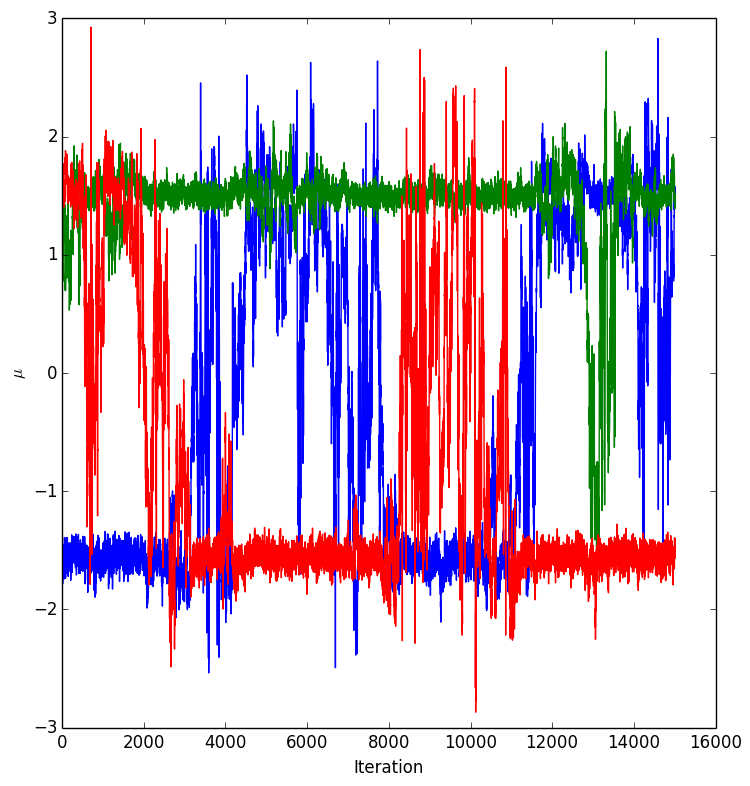
\includegraphics[width = 0.45\textwidth]{out/mu.png}
    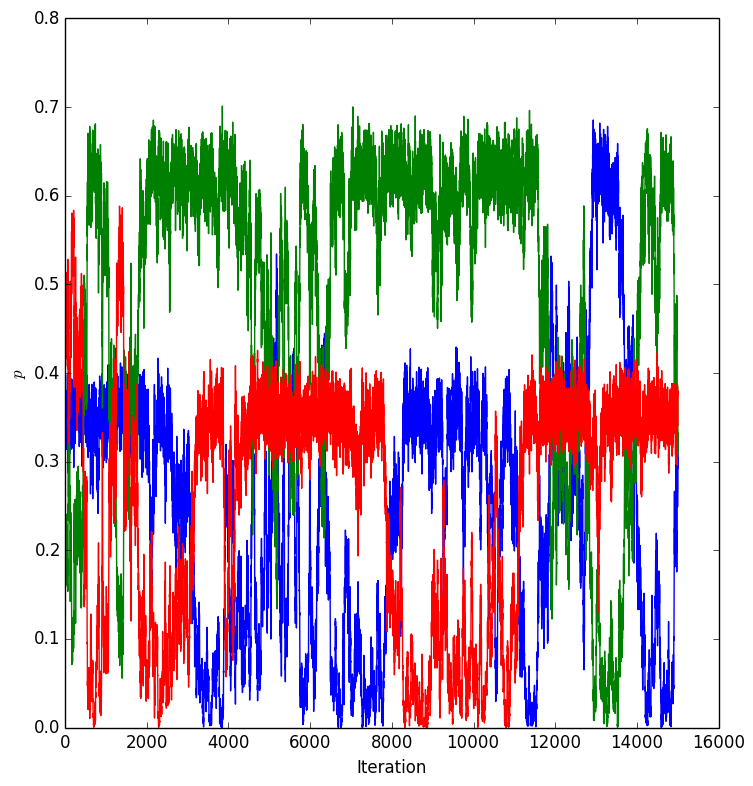
\includegraphics[width = 0.45\textwidth]{out/p.png}
    \caption{Trace plots for the sampled values of $\mu$ and $p$.
    Each component is shown in a different color.}
    \label{fig:mix.trace}
    \end{figure}

\end{document}
